\documentclass[12pt]{report}
\usepackage[a4paper,margin=1in]{geometry}
\usepackage{setspace}
\usepackage{graphicx}
\usepackage{sectsty}
\usepackage{pdfpages}
% \usepackage{booktabs}
\usepackage[export]{adjustbox}
\usepackage{amssymb}
\usepackage{cancel}
\usepackage[numbered]{matlab-prettifier}
\usepackage{circuitikz}
\usepackage{xfrac}
\usepackage{lmodern}
\usepackage{multicol}
\usepackage{caption}
\usepackage{listings}
\usepackage{amsmath}
\newcommand{\eqname}[1]{\tag*{#1}}% Tag equation with name

\usetikzlibrary{arrows}
\graphicspath{{images/}}
\usetikzlibrary{calc,patterns,angles,quotes}

\allsectionsfont{\bfseries\Large\raggedright}
\renewcommand\thesection{\arabic{section}}
\renewcommand{\thefootnote}{\arabic{footnote}}

\begin{document}

\input{titlepage}
% \tableofcontents{}
\newpage
\begin{flushleft}

\begin{multicols}{2}

\section{Objective}
In this lab the objective is to discover what forces are involved when an
object with a large mass is brought along a curved path. Observing these forces
will allow us to explore the concept of force, centripetal acceleration, and
instantanious velocity.
\section{Theory}
Throughout this lab we spun a triple beam balance to determine forces on an
observed mass. To do so, we will need a few equations.
\begin{align}
  a_c &= \frac{v^2}{r} \label{centripetal_acceleration} \\ \eqname{Centripetal Acceleration} \\
  v &= \frac{\Delta x}{\Delta t} = \frac{2\pi r}{T} \label{velocity} \\ \eqname{Velocity} \\
  r &= \frac{F_c}{4\pi^2M}T^2 \label{radius} \\ \eqname{Radius of Rotation} \\
  F_c &= Ma_c \label{centripetal_force} \\ \eqname{Centripetal Force}
\end{align}
\section{Equipment}
In this lab we will use a Centripetal Force Apparatus to determine forces on the objects on it when spun. We will use a pulley for hangin masses off of. A string will connect out masses with out machines.
Masses are to be used for every piece of equipment that mentions a mass. A mass hangas will elevate the masses for the purpose of the lab. We will use a bubble level to ensure out tooling is level. A triple beam balance will be used to determine the mass of out masses.\\ All equipment is  displayed in the Appendix.
\section{Procedure}
We begin the lab by ensuring that the center post assembly is at the center of the track.
We then adjust the leveling screws to ensure that the Apparatus is level. We then select a mass to attach to the hangar and move the side post assembly to our specified radius of 15 cm. We adjust the system to find an equilibrium point where all strings are staight. We adjust the height of the indicator bracket to match the pink disk. We remove the mass and spin the apparatus to return the pink disk to the indicator. We log data for multiple radii.
\begin{center}
\flushleft Table 1: Varying the Radius
\footnotesize
\begin{tabular}{|c|c|c|c|c|}
\hline
Trial \# & M (kg) & r (m) & $F_c = mg (N)$ & T (s) \\
1 & 0.1365 & 0.150 & 0.2418 & 1.597 \\
2 & 0.1365 & 0.170 & 0.2418 & 1.140 \\
3 & 0.1365 & 0.180 & 0.2418 & 1.101 \\
4 & 0.1365 & 0.140 & 0.2418 & 2.360 \\
5 & 0.1365 & 0.160 & 0.2418 & 1.430 \\
\hline
\end{tabular}
\end{center}
\vspace{0.5cm}
We repeat the steps above with multiple forces.
\begin{center}
\flushleft Table 2: Varying the Force
\footnotesize
\begin{tabular}{|c|c|c|c|c|}
\hline
Trial \# & M (kg) & r (m) & $F_c = mg (N)$ & T (s) \\
1 & 0.1365 & 0.160 & 0.5396 & 1.335 \\
2 & 0.1365 & 0.160 & 1.0301 & 1.000 \\
3 & 0.1365 & 0.160 & 0.7358 & 1.163 \\
4 & 0.1365 & 0.160 & 1.2263 & 0.948 \\
5 & 0.1365 & 0.160 & 0.4415 & 1.386 \\
\hline
\end{tabular}
\end{center}
\vspace{0.5cm}
We repeat the steps above with multiple masses.
\begin{center}
\flushleft Table 3: Varying the Mass
\footnotesize
\begin{tabular}{|c|c|c|c|c|}
\hline
Trial \# & M (kg) & r (m) & $F_c = mg (N)$ & T (s) \\
1 & 0.1462 & 0.160 & 0.7358 & 1.211 \\
2 & 0.1065 & 0.160 & 0.7358 & 1.045 \\
3 & 0.2063 & 0.160 & 0.7358 & 1.339 \\
\hline
\end{tabular}
\end{center}

\newpage
\section{Analysis}
\large Part 1 \\ \normalsize
We can rewrite equation (\ref{centripetal_force}) in the form
\begin{equation}
r = (\frac{F_c}{4\pi^2M})T^2
\end{equation}
It is expected that plotting r vs. $T^2$ should be a straight line $y = \alpha x$ with a slope of
$\alpha = \frac{F_c}{4\pi^2M}$. Plotting the data, we produce the following graph \\
\small Figure 1 \\
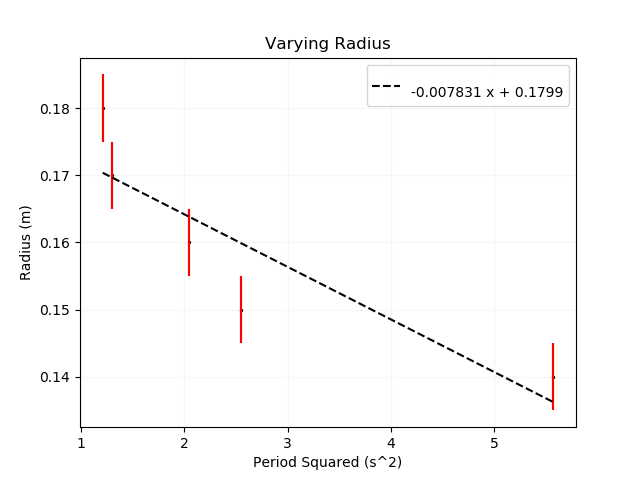
\includegraphics[scale=0.45]{VaryingRadius}
\center Radius of mass to center of rotation of the Apparatus vs. the square of the period.\\
\begin{tabular}{ll}
experimental slope: & -0.007831 \\
theoretical slope: & 0.048708 \\
percent difference: & -117.45\%
\end{tabular}
\flushleft The slope observed from our data is not consistent with our
prediction of the slope. It is possible that we had an error in our data collection
that disrupted the data. \\
\vspace{10px}
\large Part 2 \\ \normalsize
We can rewrite equation (\ref{centripetal_force}) in the form
\begin{equation} \label{centripetal_force2}
F_c = (4\pi^2Mr)\frac{1}{T^2}
\end{equation}
It is expected that plotting $F_c$ vs. $\frac{1}{T^2}$ should be a straight line $y = \alpha x$ with a slope of
$\alpha = (4\pi^2Mr)$. Plotting the data, we produce the following graph \\
\small Figure 2 \\
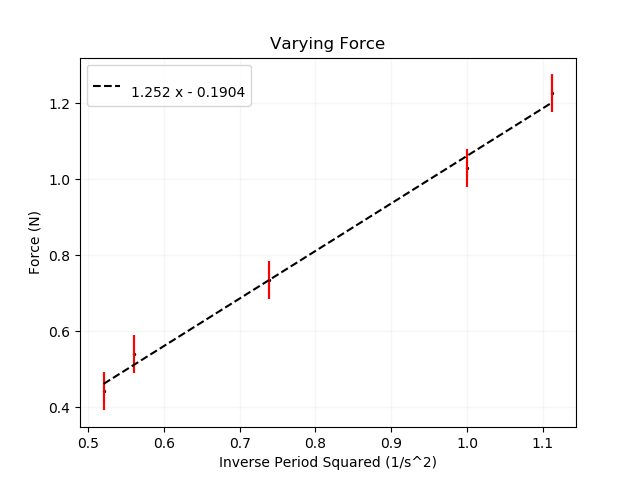
\includegraphics[scale=0.45]{VaryingForce}
\center Centripetal force (mg) induced by the spinning Apparatus vs. the inverse
of the period squared.\\
\begin{tabular}{ll}
experimental slope: & 1.252 \\
theoretical slope: & 0.862 \\
percent difference: & 45.22\%
\end{tabular}
\flushleft The slope observed from our data is not consistent with our
prediction of the slope. It is significantly closer to our theoretical slope than
when we varied the radius that the mass was spun at. This is still likely to be the result of some data collection error or experiment execution error. \\
\vspace{10px}
\large Part 3 \\ \normalsize
For our experiment where we vary the mass we use (Eq. \ref{centripetal_force2})
and compare out experimental force to (\ref{centripetal_force2})'s theoretical force.
We then calculate the percent difference. \\
\begin{center}
\flushleft Table 4: Expected and Theoretical forces \center
\begin{tabular}{|c|c|c|}
\hline
$F_{exp}$ & $F_{theoretical}$ & $\%_{diff}$ \\
0.7358 & 0.7626 & -3.51 \\
0.7358 & 0.6437 & 14.30 \\
0.7358 & 0.4732 & -24.39 \\
\hline
\end{tabular}
\end{center}

\section{Error Analysis}
In this las be experienced some large \% differences from the theoretical values that were expected. Possible sources of error arise when we look at the data collection process. We have to determine what level the pink indicator disk needs to be at for equilibrium. This is a source of error. Another source of error is determining what a complete spin is considered. This could be mitigated by an encoder attached to the apparatus that measures the angle. Manually timing is another source of error. This causes variation in out recorded times. In addition to the aforementioned encoder we could mitigate this error by choosing initial conditions that produce a large period. This reduces the fractional error from hand timing.

\section{Conclusion}
The purpose of this lab was to experimentally observe the variable that influence centripetal force. The results we got mainly supported the formula that we were testing but our varying radius experiment failed to support out formulas due to human error. From this lab we were able to determine the effects of radius and mass on the centripetal force of a spinning object.
\end{multicols}
\section{Appendix}
\begin{large}
Full Sized Figures \\
\end{large}
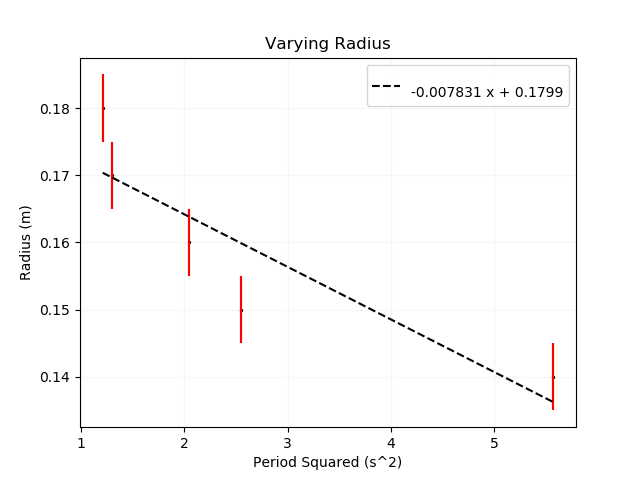
\includegraphics{VaryingRadius}
\begin{center}
  Figure 1: Varying Radius
\end{center}
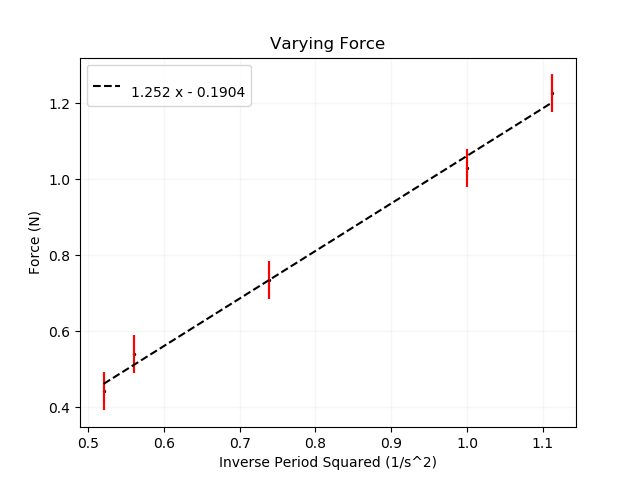
\includegraphics{VaryingForce}
\begin{center}
  Figure 2: Varying Force
\end{center}
\begin{large}
\newpage
Equipment Sketches \\
\end{large}
\begin{center}
  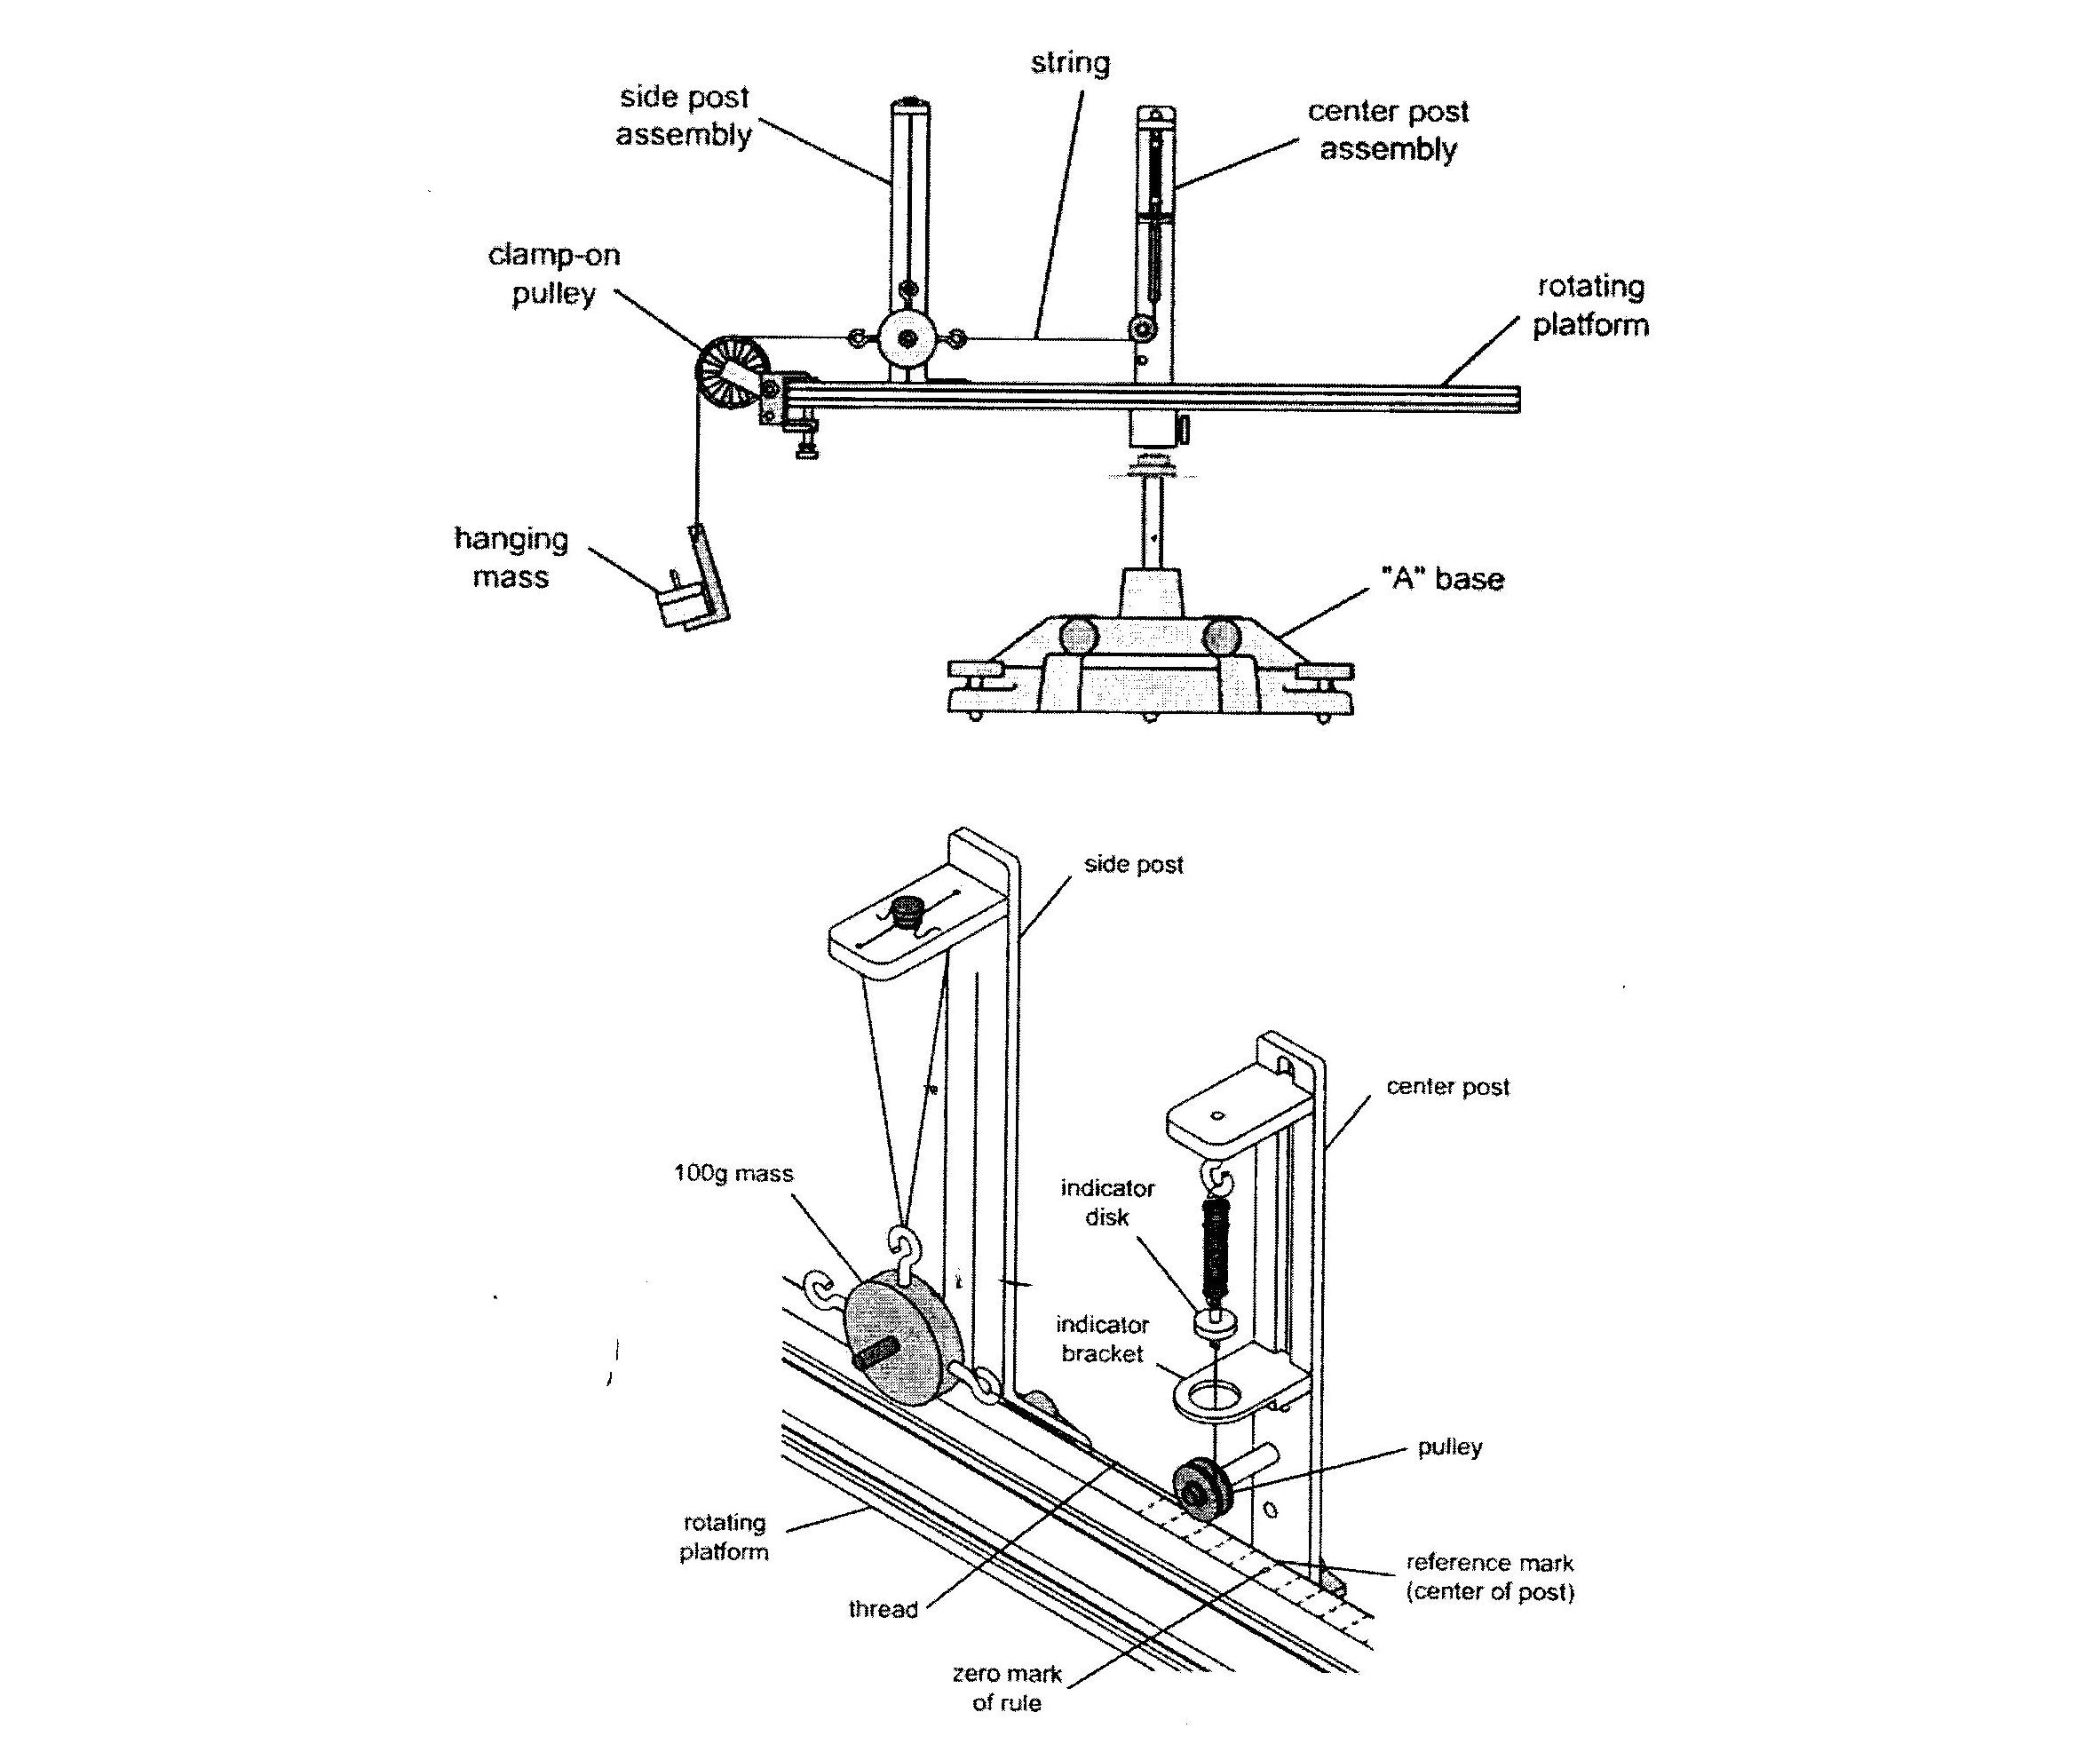
\includegraphics[scale=0.2]{equipment1}
  Figure 3: Spinning Apparatus
\end{center}
\newpage
\begin{large}
\end{large}
Lab Code \\
\begin{lstlisting}
import numpy as np
from scipy import stats
import matplotlib.pyplot as plt

#Varying the radius
plt.figure("Varying Radius")
r = np.array([0.15, 0.17, 0.18, 0.14, 0.16])
t = np.array([1.597, 1.14, 1.101, 2.36, 1.43])
t_squared = t**2
goal_slope = 0.2418/(4*np.pi**2*0.1365) #Fc/(4pi^2M)T^2
x,y = t_squared,r
plt.scatter(x,y, c='r', s=5)

best_fit = np.poly1d(np.polyfit(x, y, 1))
actual_slope = best_fit.c[0]
best_fit_s = str(best_fit)

plt.plot(np.unique(x), np.poly1d(np.polyfit(x, y, 1))(np.unique(x)), 'k--',
label=best_fit_s)
plt.legend()

plt.title('Varying Radius')
plt.xlabel('Period Squared (s^2)')
plt.ylabel('Radius (m)')

print(f'''
Varying Radius
The ideal slope is {goal_slope}
The actual slope is {actual_slope}
The percent difference is {(actual_slope-goal_slope)/goal_slope*100}%
    ''')
plt.savefig('VaryingRadius.png')

#Varying the force
plt.figure("Varying Force")
f = np.array([0.5396, 1.0301, 0.7358, 1.2263, 0.4415])
t = np.array([1.335, 1, 1.163, 0.948, 1.386])
inverse_t_squared = 1/(t**2)
goal_slope = 4*np.pi**2*0.1365*0.16 #4pi^2Mr * 1/T^2

x,y = inverse_t_squared,f
plt.scatter(x,y, c='r', s=5)

best_fit = np.poly1d(np.polyfit(x, y, 1))
actual_slope = best_fit.c[0]
best_fit_s = str(best_fit)

plt.plot(np.unique(x), np.poly1d(np.polyfit(x, y, 1))(np.unique(x)), 'k--',
label=best_fit_s)
plt.legend()

plt.title('Varying Force')
plt.xlabel('Inverse Period Squared (1/s^2)')
plt.ylabel('Force (N)')

print(f'''
Varying Force
The ideal slope is {goal_slope}
The actual slope is {actual_slope}
The percent difference is {(actual_slope-goal_slope)/goal_slope*100}%
    ''')
plt.savefig('VaryingForce.png')



#Varying the mass
m = np.array([0.1462, 0.1065, 0.2063])
t = np.array([1.211, 1.045, 1.339])
f = 0.7358
for index in range(3):
    expected_force = 4*np.pi**2*m[index]*0.16/t[index]
    print(f'''
Varying Mass
The ideal mass is {expected_force}
The actual slope is {f}
The percent difference is {(f-expected_force)/expected_force*100}%
    ''')


plt.ion()
plt.show()
plt.pause(10)
\end{lstlisting}

\end{flushleft}
\end{document}
